\section{Analysis of Outcomes}
\label{sec:outcome}

\subsection{Preprocessing}
Before we get down to read all data into our workbench in R, we need to preprocess the file format so as to delete some redundant data and adjust the format of some fields. Generally, out preprocessing includes the following steps:
\begin{itemize}
  \item \textbf{Delete Redundant Data}. For instances, the field \texttt{instant} in  Table~\ref{tab:fields} only records the indexes of data entries, which should be eliminated from the data manipulation.
  \item \textbf{Format Transformation}. The data format of some fields should be transformed, especially some \emph{qualitative} fields such as \texttt{weathersit} and \texttt{holiday}, so that R language could recognize them as qualitative variables and create dummy variables.
\end{itemize}

We use a simple python script to preprocess the input file, which is provided in Section~\ref{apd:pre} in appendix. After preprocessing, there are totally 15 variables left in the model, the deleted ones are labeled as {\color{red}red} and the transformed ones are labeled as {\color{green}green} in Table~\ref{tab:fields}.

\subsection{Fit all Linear Variables}
\label{sec:fitall}
In the remaining 15 variables, we first fit all predictors in linear form and the response is \texttt{cnt}:
\begin{lstlisting}[style=rlanguage]
>lm.fit_all = lm(cnt~.-registered-casual,data=bicycle)
>summary{lm.fit_all}

Call:
lm(formula = cnt ~ . - registered - casual, data = bicycle)

Residuals:
    Min      1Q  Median      3Q     Max
-396.57  -60.52   -7.94   51.34  440.09

Coefficients:
               Estimate Std. Error t value Pr(>|t|)
(Intercept)    -50.9441     8.9203  -5.711 1.14e-08 ***
seasonSpring   -32.0083     5.7453  -5.571 2.57e-08 ***
seasonSummer     6.2138     4.9737   1.249  0.21156
seasonWinter    35.9871     5.1574   6.978 3.11e-12 ***
.....
---
Signif. codes:  0 ‘***’ 0.001 ‘**’ 0.01 ‘*’ 0.05 ‘.’ 0.1 ‘ ’ 1

Residual standard error: 101.7 on 17330 degrees of freedom
Multiple R-squared:  0.6863,	Adjusted R-squared:  0.6855
F-statistic:   790 on 48 and 17330 DF,  p-value: < 2.2e-16
\end{lstlisting}
From the summary we could see that R language has calculated the slope and intercept for all input linear predictors, besides, it also creates dummy variables for qualitative predictors like \texttt{seasonSpring}, \texttt{seasonSummer}. For detailed information about dummy variables, we can use \texttt{Contrasts} function.

\begin{lstlisting}[style=rlanguage]
> contrasts(season)
       Spring Summer Winter
Autumn      0      0      0
Spring      1      0      0
Summer      0      1      0
Winter      0      0      1
\end{lstlisting}

The result shows that $F-statistic = 729.1$ and $p-value < 2.2e-16$ thus there \textbf{is} a relationship between the predictors and the response \texttt{cnt}.

Nevertheless, the summary also demonstrates that not all predictors have strong relationship with the response \texttt{cnt} (high p-value). We may wish to run a regression without these predictors. Furthermore, we have not taken interaction terms and quadratic predictors into consideration.

\subsection{Interactive Predictors}
\label{sec:interactive}
In order to explore the interactive relationships amongst predictors, we plot the \texttt{Scatterplot Matrix} of quantitative predictors as shown in Figure~\ref{fig:interactive}.

\begin{figure}
  \centering
  % Requires \usepackage{graphicx}
  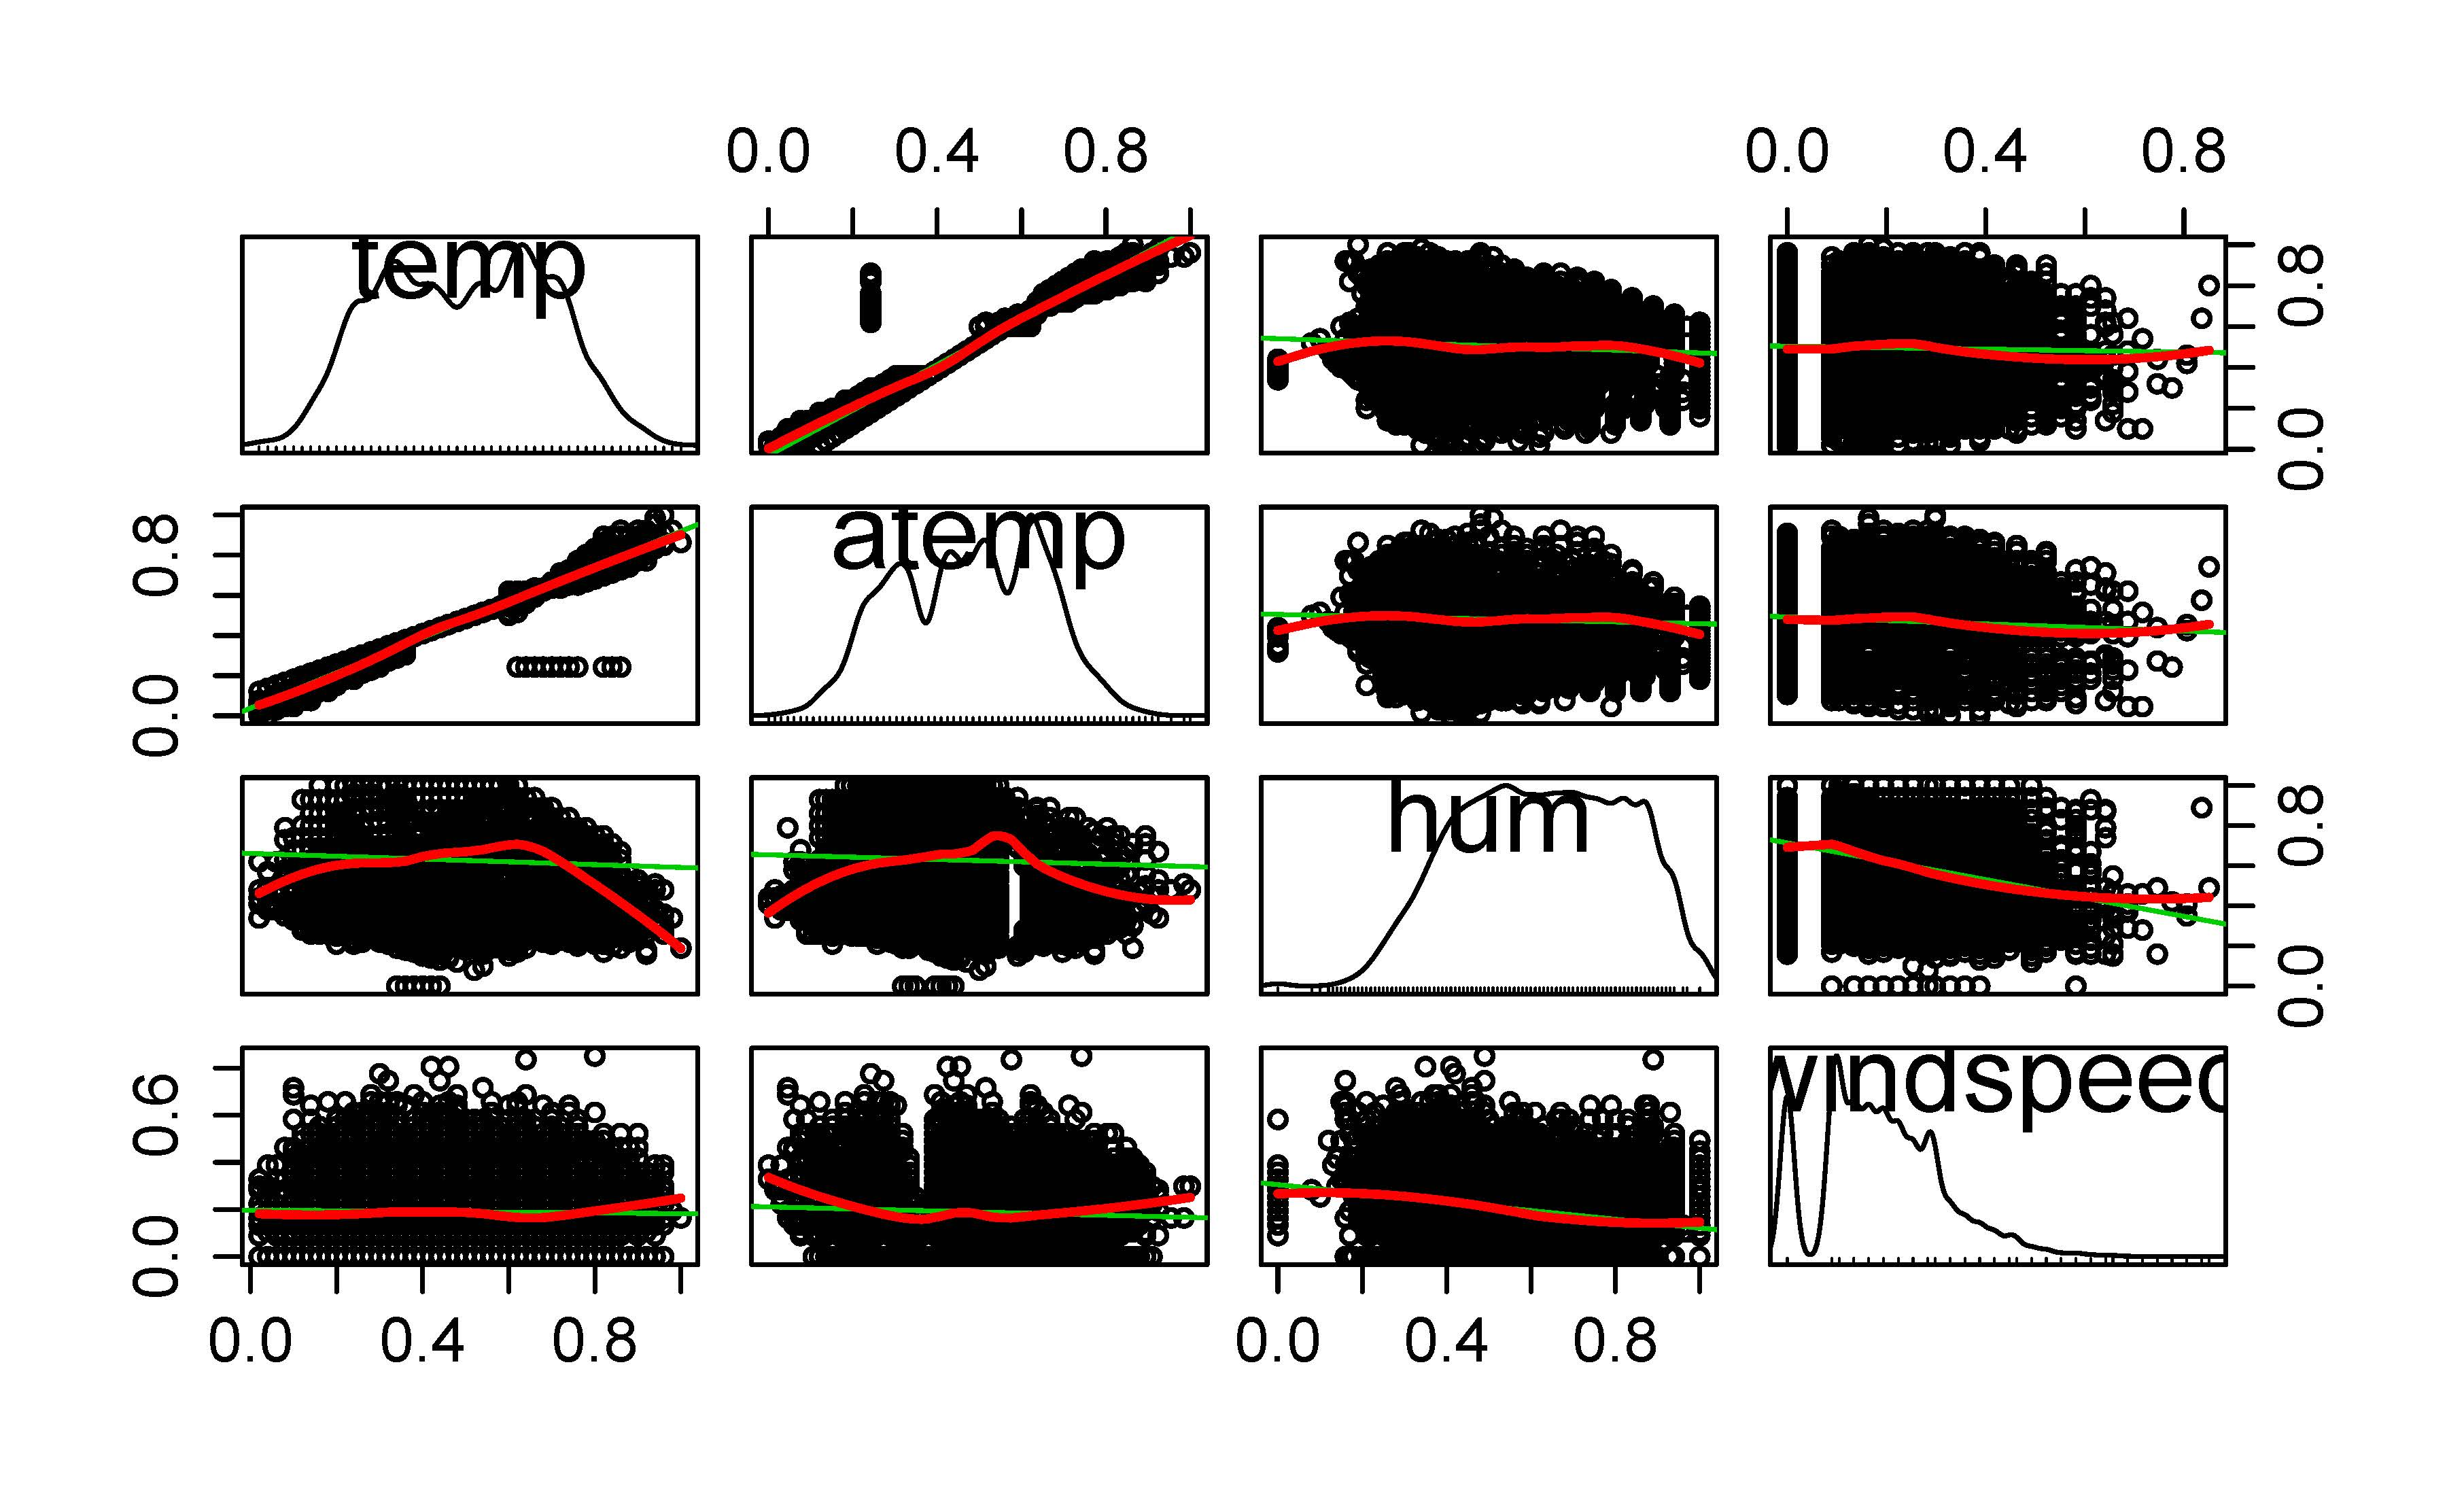
\includegraphics[width=\linewidth]{pic/interactive.jpg}\\
  \caption{Scatter graphs amongst the predictors}\label{fig:interactive}
\end{figure}
From the graph we could find that there are obvious interactive relationships between \texttt{temp} and \texttt{atemp}. Thus we may need to exclude one of them in the following model.
Now we should take interactive predictors into account.
\begin{lstlisting}[style=rlanguage]
> lm.fit_interactive = lm(cnt~season+yr+mnth+hr+holiday+weekday+workingday+weathersit+(temp+atemp+hum+windspeed)^2,data=bicycle)
> summary(lm.fit_interactive)

Call:
lm(formula = cnt ~ season + yr + mnth + hr + holiday + weekday +
    workingday + weathersit + (temp + atemp + hum + windspeed)^2,
    data = bicycle)

Residuals:
    Min      1Q  Median      3Q     Max
-387.90  -59.54   -6.05   50.61  440.80

Coefficients: (1 not defined because of singularities)
                Estimate Std. Error t value Pr(>|t|)
(Intercept)     -135.218     15.560  -8.690  < 2e-16 ***
seasonSpring     -31.085      5.732  -5.423 5.93e-08 ***
seasonSummer       8.286      4.963   1.669 0.095072 .
seasonWinter      34.792      5.157   6.746 1.57e-11 ***
...
temp             363.461    116.997   3.107 0.001896 **
atemp             89.101    136.020   0.655 0.512440
hum               78.731     17.513   4.495 6.99e-06 ***
windspeed        -97.118     28.806  -3.371 0.000749 ***
temp:atemp       -76.967     29.540  -2.605 0.009182 **
temp:hum        -430.001    150.277  -2.861 0.004223 **
temp:windspeed   207.574    212.509   0.977 0.328692
atemp:hum         98.317    173.577   0.566 0.571120
atemp:windspeed  -24.759    237.449  -0.104 0.916957
hum:windspeed    -18.163     32.638  -0.557 0.577868
---
Signif. codes:  0 ‘***’ 0.001 ‘**’ 0.01 ‘*’ 0.05 ‘.’ 0.1 ‘ ’ 1

Residual standard error: 100.9 on 17320 degrees of freedom
Multiple R-squared:  0.6914,	Adjusted R-squared:  0.6903
F-statistic: 668.9 on 58 and 17320 DF,  p-value: < 2.2e-16
\end{lstlisting}

The result shows that Residual standard error (RSE) has decreased to 100.9 thus there does exist some interactive predictors like \texttt{temp:atemp} with $p-value < 0.01$. However, the summary also reveals that most interactive predictors are not strong enough (p-values are high). These interactive predictors should eliminated from the final regression.

\subsection{Non-linear Predictors}
\label{sec:non-linear}
The model may involve some non-linear predictors. For simplicity, we only consider the quadratic situation initially.
\begin{lstlisting}[style=rlanguage]
> lm.fit_quad = lm(cnt~season+yr+mnth+hr+holiday+weekday+workingday+weathersit+(temp+atemp+hum+windspeed)^2+I(temp^2)+I(atemp^2)+I(hum^2)+I(windspeed^2),data=bicycle)
> summary(lm.fit_quad)

Call:
lm(formula = cnt ~ season + yr + mnth + hr + holiday + weekday +
    workingday + weathersit + (temp + atemp + hum + windspeed)^2 +
    I(temp^2) + I(atemp^2) + I(hum^2) + I(windspeed^2), data = bicycle)

Residuals:
    Min      1Q  Median      3Q     Max
-368.60  -59.80   -6.16   50.63  426.48

Coefficients: (1 not defined because of singularities)
                 Estimate Std. Error t value Pr(>|t|)
(Intercept)     -239.6372    20.3619 -11.769  < 2e-16 ***
seasonSpring     -32.5150     5.7159  -5.689 1.30e-08 ***
seasonSummer       7.1233     4.9525   1.438  0.15036
seasonWinter      34.4370     5.1419   6.697 2.19e-11 ***
...
I(temp^2)       -172.4633   191.0114  -0.903  0.36659
I(atemp^2)       254.3896   163.2068   1.559  0.11909
I(hum^2)        -178.6966    22.2267  -8.040 9.58e-16 ***
I(windspeed^2)  -239.4821    38.8895  -6.158 7.53e-10 ***
temp:atemp      -161.7557   272.5325  -0.594  0.55284
temp:hum        -417.9212   161.5882  -2.586  0.00971 **
temp:windspeed   463.6974   229.8050   2.018  0.04363 *
atemp:hum         27.0760   183.6174   0.147  0.88277
atemp:windspeed -311.4761   256.8682  -1.213  0.22530
hum:windspeed   -167.8291    36.2282  -4.633 3.64e-06 ***
---
Signif. codes:  0 ‘***’ 0.001 ‘**’ 0.01 ‘*’ 0.05 ‘.’ 0.1 ‘ ’ 1

Residual standard error: 100.6 on 17316 degrees of freedom
Multiple R-squared:  0.6935,	Adjusted R-squared:  0.6924
F-statistic:   632 on 62 and 17316 DF,  p-value: < 2.2e-16
\end{lstlisting}

Amongst the four quantitative predictors (\texttt{temp, atemp, windspeed, hum}), we find \texttt{hum} and \texttt{windspeed} has a quadratic linear relationship with the response. We now try to find linear relationships with higher order using \texttt{poly}.
\begin{lstlisting}[style=rlanguage]
poly(hum, 5)1             NA         NA      NA       NA
poly(hum, 5)2       -979.025    115.517  -8.475  < 2e-16 ***
poly(hum, 5)3        338.896    104.027   3.258  0.00113 **
poly(hum, 5)4        274.301    104.738   2.619  0.00883 **
poly(hum, 5)5        130.117    102.407   1.271  0.20389
poly(windspeed, 5)1       NA         NA      NA       NA
poly(windspeed, 5)2 -726.289    113.764  -6.384 1.77e-10 ***
poly(windspeed, 5)3 -104.216    102.027  -1.021  0.30705
poly(windspeed, 5)4  -29.970    102.149  -0.293  0.76923
poly(windspeed, 5)5  -47.567    101.215  -0.470  0.63839
\end{lstlisting}
The results shows that the linear, quadratic, cubic and quartic form of \texttt{hum} all have a relationship with the response and only the quadratic form of \texttt{windspeed} has significant p-value in regression fit.

\subsection{Backward Selection}
Now we should adjust the model and eliminate some redundant predictors to refine the model.
\begin{lstlisting}[style=rlanguage]
> lm.fit_fin = lm(cnt~season+yr+mnth+hr+holiday+weekday+weathersit+(temp+hum+windspeed)^2+poly(hum,4)+I(windspeed^2),data=bicycle)
> summary(lm.fit_fin)

Call:
lm(formula = cnt ~ season + yr + mnth + hr + holiday + weekday +
    weathersit + (temp + hum + windspeed)^2 + poly(hum, 4) +
    I(windspeed^2), data = bicycle)

Residuals:
    Min      1Q  Median      3Q     Max
-366.40  -59.41   -5.70   50.19  424.33

Coefficients: (1 not defined because of singularities)
               Estimate Std. Error t value Pr(>|t|)
(Intercept)    -150.337     13.187 -11.400  < 2e-16 ***
seasonSpring    -31.664      5.699  -5.556 2.80e-08 ***
seasonSummer      8.979      4.925   1.823  0.06831 .
seasonWinter     35.209      5.115   6.883 6.06e-12 ***
...
temp:hum       -340.669     24.058 -14.161  < 2e-16 ***
temp:windspeed  190.288     35.142   5.415 6.21e-08 ***
hum:windspeed  -181.499     35.112  -5.169 2.38e-07 ***
---
Signif. codes:  0 ‘***’ 0.001 ‘**’ 0.01 ‘*’ 0.05 ‘.’ 0.1 ‘ ’ 1

Residual standard error: 100.6 on 17320 degrees of freedom
Multiple R-squared:  0.6933,	Adjusted R-squared:  0.6923
F-statistic: 675.1 on 58 and 17320 DF,  p-value: < 2.2e-16
\end{lstlisting}

The final model suggests that RSE = 100.6. This model could depict the relationship between the predictors and response \texttt{cnt} to some extent.

\subsection{Transformation of Temporal Variable}
To investigate the effect of temporal variables (\texttt{hr, yr, mnth}...), we have also implemented a version of {\mlr} which takes these predictors as continuous variable. Considering the temporal data in the given data file could only provide an accuracy of hours, we use the \texttt{instant} fields in the file to represent how many hours since 2011/1/1 00:00.
\begin{lstlisting}[style=rlanguage]
> lm.fit_time = lm(cnt~((.-registered-casual)^2+I(time^2)),data=bicycle_time)
> summary(lm.fit_time)

Call:
lm(formula = cnt ~ ((. - registered - casual)^2 + I(time^2)),
    data = bicycle_time)

Residuals:
    Min      1Q  Median      3Q     Max
-408.54  -90.43  -23.63   61.12  656.88

Coefficients: (34 not defined because of singularities)
                               Estimate Std. Error t value Pr(>|t|)
(Intercept)                   2.270e+02  6.271e+01   3.620 0.000295 ***
time                          1.632e-03  2.804e-03   0.582 0.560590
...
atemp:hum                     6.222e+02  2.987e+02   2.083 0.037239 *
atemp:windspeed               2.507e+02  3.637e+02   0.689 0.490755
hum:windspeed                 1.976e+02  5.709e+01   3.461 0.000539 ***
---
Signif. codes:  0 ‘***’ 0.001 ‘**’ 0.01 ‘*’ 0.05 ‘.’ 0.1 ‘ ’ 1

Residual standard error: 143 on 17242 degrees of freedom
Multiple R-squared:  0.383,	Adjusted R-squared:  0.3781
F-statistic: 78.68 on 136 and 17242 DF,  p-value: < 2.2e-16
\end{lstlisting}

From the summary we could see that the RSE is 143, higher than the model which takes temporal variables as qualitative predictors. Thus it is inappropriate to transform time into contiguous values in this regression.


